% Résumé du principe de l'expérience

Au cours de l'expérience, nous allons mesurer le champ magnétique dans un solénoïde en faisant varier le nombre de spires, ainsi qu'en des point décalé du centre de celui-ci afin de voir les variations du champs dans les bords.

\subsection{Matériel}
% Liste du matériel

Le matériel suivant a été nécessaire a la réalisation de cette expérience:\\
\begin{itemize}
	\item Un générateur
	\item Un teslamètre
	\item Un solénoïde 
	\item 2 câbles
\end{itemize}

\subsection{Déroulement}
% Déroulement de l'expérience

Il est nécessaire d'assembler le dispositif d'expérimentation (voir le schéma ci-dessous) avant les manœuvres suivantes.\\
Il est important d'insérer le teslamètre dans le solénoïde, et s'assurer que le bout de ce dernier soit au centre (marqueur sur le solénoïde aligné avec le $0$ sur la réglette du teslamètre). De plus, il faut paramétrer le teslamètre pour que le bruit ne soit pas présent dans la mesure, soit qu'il affiche $0 \ [T]$.\\

\paragraph{Première expérience :}
\begin{itemize}
    \item Mesurer le champ en augmentant le nombre de spires (5, 10, 20, 30, 50, 70, puis 100 spires). Cela se fait en augmentant la distance parcouru par le courant dans la bobine.
    \item Prendre note de la puissance du champ.\\
\end{itemize}

\paragraph{Deuxième expérience :}
\begin{itemize}
    \item On commence par utiliser 20 spires.
    \item Tirer le teslamètre de 1 en 1 $[cm]$ jusqu'à l'extrémité du solénoïde en prenant note de la puissance du champ en chaque point.
    \item Faire de même avec 50 et 100 spires.\\
\end{itemize}

\subsection{Schéma}
% Schéma avec légende

\begin{figure}[H]
  \centering
    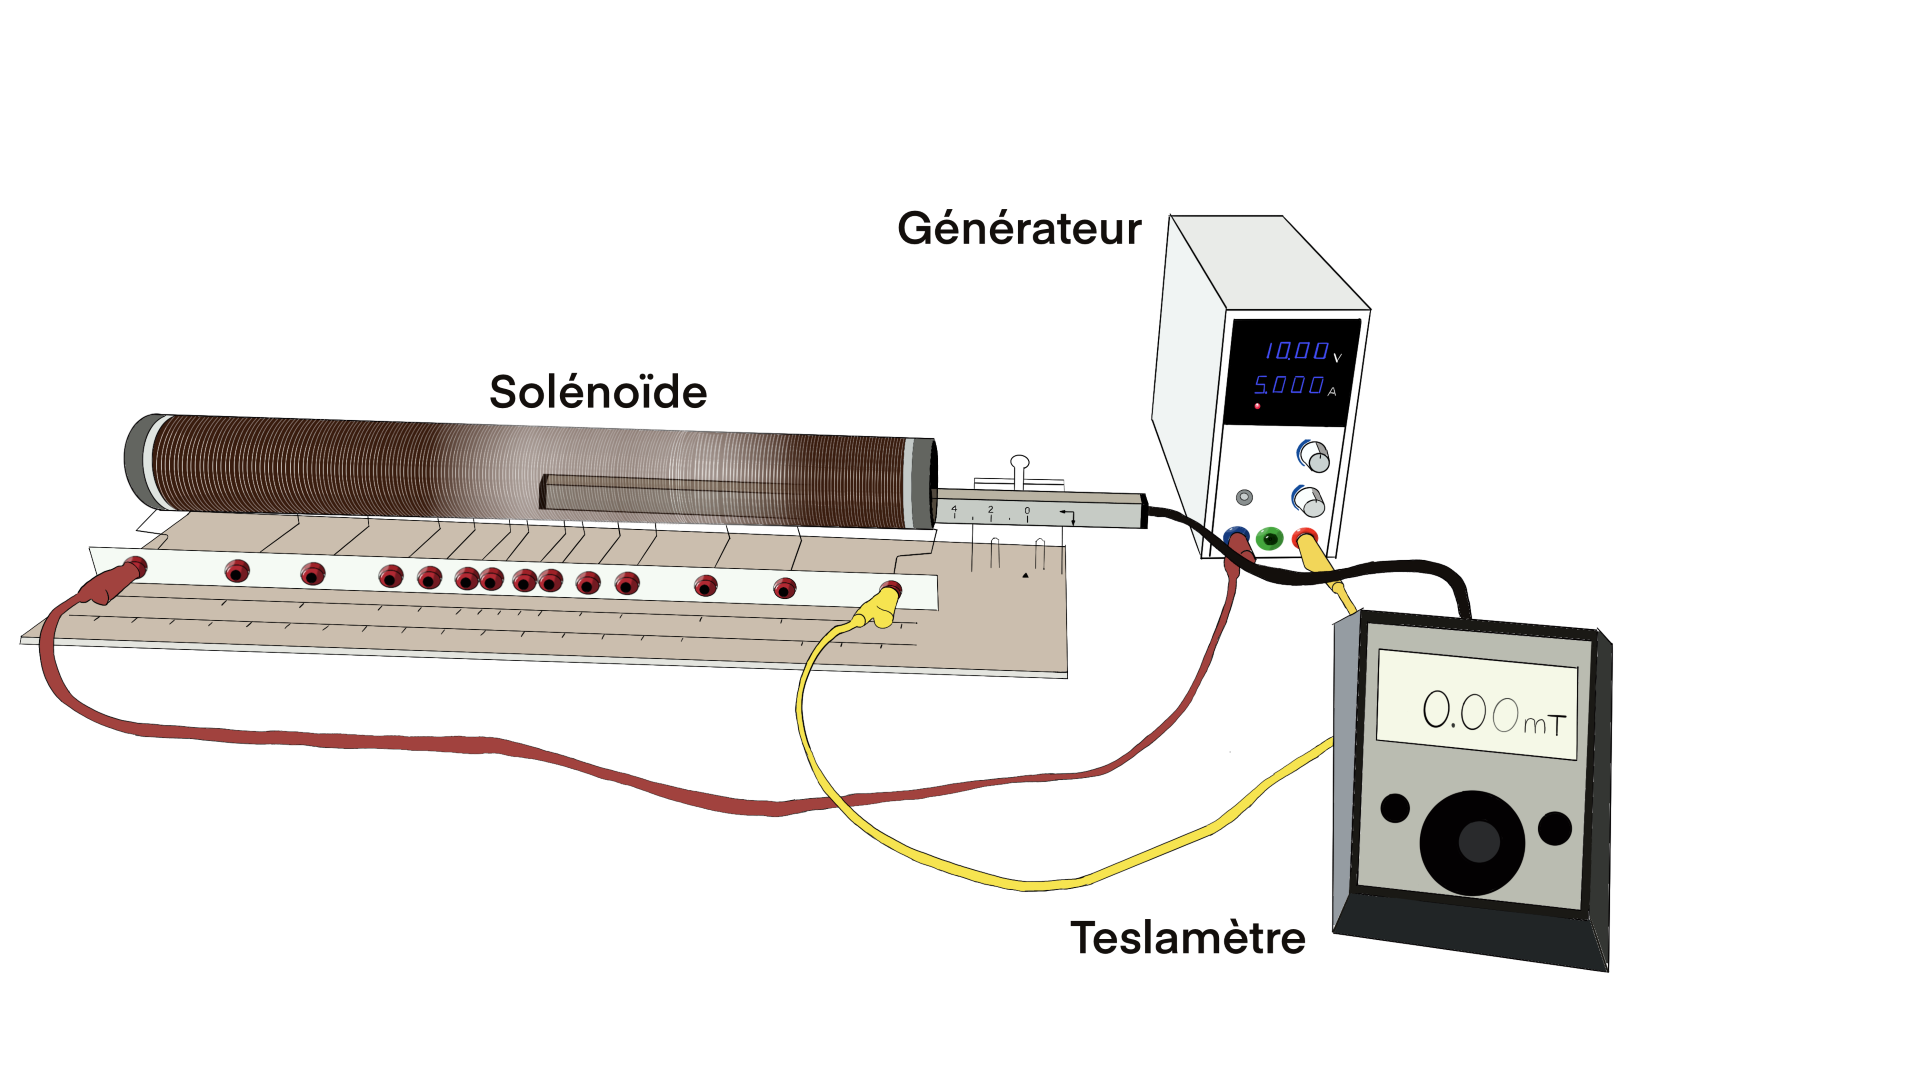
\includegraphics[width=1\textwidth]{Sol_schéma}
\end{figure}